\problemname{Skolvägen}

\begin{figure}[!h]
\begin{center}
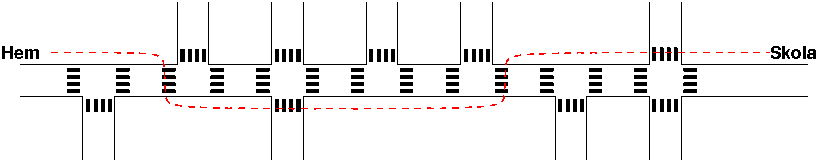
\includegraphics[width=0.8\textwidth]{skolvag.png}
\end{center}
\caption{Den streckade linjen visar Cissis väg i första exemplet.}
\end{figure}

\noindent
Cissi går från sitt hem till skolan längs en lång gata som går i väst-östlig riktning.
På sin väg passerar hon ett antal korsningar där tvärgator utgår norrut (\texttt{N}), söderut (\texttt{S}) eller både norrut och söderut (\texttt{B}).
Vid varje korsning finns övergångsställen på både tvärgator och huvudgata (se figuren ovan), och dessa måste givetvis följas.

Både hemmet och skolan ligger på norra sidan av gatan.
Skriv ett program som hjälper Cissi att beräkna det minsta antalet gator hon måste korsa på sin väg till skolan. 

\section*{Indata}
Indata består av en enda rad med högst $1\,000$ bokstäver, som vardera är {\tt N}, {\tt S} eller {\tt B}.
Bokstäverna beskriver korsningarna i precis den ordning som Cissi passerar dem.

\section*{Utdata}
En rad med ett heltal, det minsta antalet gator Cissi behöver korsa.

\section*{Poängsättning}
Ditt program kommer att testas på $5$ testfall.
För varje testfall som du klarar får du $20$ poäng.

För testfall värda $40$ poäng kommer antalet bokstäver vara högst $20$.
